\documentclass{standalone}
\usepackage{../preamble}

\begin{document}
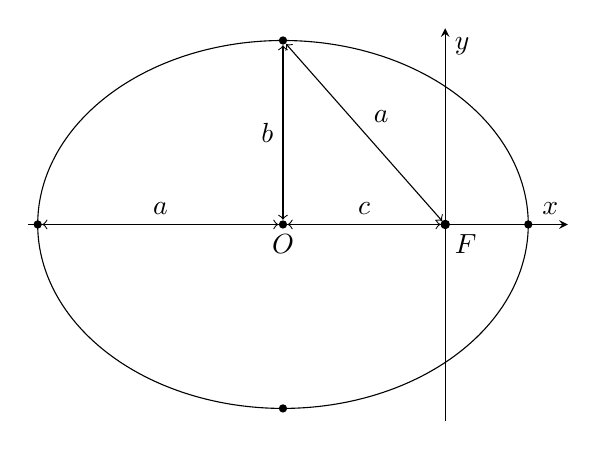
\begin{tikzpicture}
  \begin{axis}[
      xmax=1,xmin=-3.4,
      ymax=1.6,ymin=-1.6,
      axis lines=middle,
      ytick = {0},
      xtick = {0},
      axis equal image,
      ylabel={$y$},
      xlabel={$x$},
    ]
    \def\a{2}
    \def\b{1.5}
    \def\c{sqrt(\a^2-\b^2)}
    \def\e{sqrt(1-\b^2/\a^2)}
    \addplot[thin,samples=400,domain=0:360] ({\a*cos(x)-\c},{\b*sin(x)});

    \draw[thin,dotted] ({-\c},\b) -- ({-\c},{\b});
    \filldraw[circle, fill=black] (0,0) circle(1.5pt);

    \node[circle,fill=black,inner sep=0pt,minimum height=3pt](F) at (0,0){};
    \node[circle,fill=black,inner sep=0pt,minimum height=3pt](A) at ({\a-\c},0){};
    \node[circle,fill=black,inner sep=0pt,minimum height=3pt](A') at ({-\a-\c},0){};
    \node[circle,fill=black,inner sep=0pt,minimum height=3pt](B) at ({-\c},{\b}){};
    \node[circle,fill=black,inner sep=0pt,minimum height=3pt](B') at ({-\c},{-\b}){};
    \node[circle,fill=black,inner sep=0pt,minimum height=3pt](C) at ({-\c},0){};
    \node[anchor=north west] at (F){$F$};
    \node[anchor=north] at (C){$O$};
    \draw[thin,<->] (A') -- (C) node[anchor=south,pos=0.5]{$a$};
    \draw[thin,<->] (B) -- (F) node[anchor=south west,pos=0.5]{$a$};
    \draw[thin,<->] (B) -- (C) node[anchor=east,pos=0.5]{$b$};
    \draw[thin,<->] (F) -- (C) node[anchor=south,pos=0.5]{$c$};
    \node[anchor=east] at ({\a^2/\c-\c},1){$\ell$};

  \end{axis}
\end{tikzpicture}
\end{document}